\documentclass[acmtog, authorversion]{acmart}

\usepackage{booktabs} % For formal tables

\usepackage[ruled]{algorithm2e} % For algorithms
\renewcommand{\algorithmcfname}{ALGORITHM}
\SetAlFnt{\small}
\SetAlCapFnt{\small}
\SetAlCapNameFnt{\small}
\SetAlCapHSkip{0pt}
\IncMargin{-\parindent}

% Metadata Information
% \acmJournal{TOG}
% \acmVolume{9}
% \acmNumber{4}
% \acmArticle{39}
% \acmYear{2010}
% \acmMonth{3}

% Copyright
%\setcopyright{acmcopyright}
%\setcopyright{acmlicensed}
%\setcopyright{rightsretained}
%\setcopyright{usgov}
\setcopyright{usgovmixed}
%\setcopyright{cagov}
%\setcopyright{cagovmixed}

% DOI
% \acmDOI{0000001.0000001_2}

% Paper history
% \received{February 2007}
% \received{March 2009}
% \received[final version]{June 2009}
% \received[accepted]{July 2009}


% Document starts
\begin{document}
% Title portion
\title{TBD}
\author{Mengying Sun}
\orcid{1234-5678-9012-3456}
\affiliation{%
  \institution{Michigan State University}
  \department{Department of Computer Science and Engineering}
  \streetaddress{104 Jamestown Rd}
  \city{East Lansing}
  \state{MI}
  \postcode{00000}
  \country{USA}}
\author{Xiaoran Tong}
\affiliation{%
  \institution{Michigan State University}
  \department{Department of Epidemiology and Biostatistics}
  \streetaddress{909 Fee Rd}
  \city{East Lansing}
  \state{MI}
  \postcode{48824}
  \country{USA}
}

\renewcommand\shortauthors{Zhou, G. et al}

\begin{abstract}
  Through this project we seek to predict complex human phenotypes from high dimensional whole genome profiles. To solve the curse of dimensionality, we adopted a two tier modeling by first choosing representative features from chromosome LD blocks, then build a higher tier predictive model upon the first tier output. We expect improvement of predictive accuracy over existing GWAS or kernel based models.
\end{abstract}


%
% The code below should be generated by the tool at
% http://dl.acm.org/ccs.cfm
% Please copy and paste the code instead of the example below. 
%
% \begin{CCSXML}
% <ccs2012>
%  <concept>
%   <concept_id>10010520.10010553.10010562</concept_id>
%   <concept_desc>Computer systems organization~Embedded systems</concept_desc>
%   <concept_significance>500</concept_significance>
%  </concept>
%  <concept>
%   <concept_id>10010520.10010575.10010755</concept_id>
%   <concept_desc>Computer systems organization~Redundancy</concept_desc>
%   <concept_significance>300</concept_significance>
%  </concept>
%  <concept>
%   <concept_id>10010520.10010553.10010554</concept_id>
%   <concept_desc>Computer systems organization~Robotics</concept_desc>
%   <concept_significance>100</concept_significance>
%  </concept>
%  <concept>
%   <concept_id>10003033.10003083.10003095</concept_id>
%   <concept_desc>Networks~Network reliability</concept_desc>
%   <concept_significance>100</concept_significance>
%  </concept>
% </ccs2012>  
% \end{CCSXML}

% \ccsdesc[500]{Computer systems organization~Embedded systems}
% \ccsdesc[300]{Computer systems organization~Redundancy}
% \ccsdesc{Computer systems organization~Robotics}
% \ccsdesc[100]{Networks~Network reliability}

%
% End generated code
%

% We no longer use \terms command
\terms{AI, Algorithms, Performance}

\keywords{ReLU}


\thanks{This work is supported by the National Science Foundation,
  under grant CNS-0435060, grant CCR-0325197 and grant EN-CS-0329609.

  Author's addresses: G. Zhou, Computer Science Department, College of
  William and Mary; Y. Wu {and} J. A. Stankovic, Computer Science
  Department, University of Virginia; T. Yan, Eaton Innovation Center;
  T. He, Computer Science Department, University of Minnesota; C.
  Huang, Google; T. F. Abdelzaher, (Current address) NASA Ames
  Research Center, Moffett Field, California 94035.}


\maketitle

\newcommand{\bs}[1]{\boldsymbol{#1}}
\section{Introduction}
The prediction of complex phenotypes from whole genome profile is still far from satisfactory, leaving large gaps between empirical heritability measured by classic pedigree studies and contemporary kernel based whole genome predictive methods that pools huge number of features across the entire genome \cite{WGP:Gustavo, WGP:Zhang, GCTA, WGP:GMatrix1, WGP:Review1}. Among popular proposals, some attribute the ``missing heritability'' to violation of the overly strong assumption that genomic effect are additve, that is, phenotype y is linked to the linear combination of genomic features $G$ or limited expanion $\bs{\phi}(G)$. The violation of linearity and between feature independence are frequently violated, demonstrable by association rules detected by screening tuples of features combinations \cite{GWA:GMDR, GWA:MDR}. To tackle non-linearity and feature combinations into prediction modeling, the recent trend of machine learning suggests multi-layered neural network (NN) that regained popularity around 2006 through a pre-training procedures \cite{DL:Intro1}, and pushed to a new depth by replacing the classical sigmoid activation to rectified linear unit (ReLU) \cite{DL:Relu1}. However, a typical NN for genomic prediction is computationally intractable due to the sheer size of the profile easily breaching the order of tens of millions features thanks to the next generation sequencing technology \cite{NGS1}.

To contruction NN predictor on genomic profiles, it is desirable to design dimensionality reduction prior to train the whole genome NN. A widely practices technique in the field of whole genome association stduies (GWA) is to drop the bulk of rare or extremely rare features in the population, that is, only a handful of individuals has non-zero values in nearly 90\% of the features. Even after such selection, the size of the profiles are till in the order of millions. Another useful characteristic of genome is that features closely located in a chromosome segment are highly correlated due to the chemical bounds between nucleotides - a phenomenon known as linkage disequilibrium (LD) \cite{LD:Intro1, LD:Haploview}. More formally, LD states that the frequency of observing a particular type of feature variation at one site is not independent to the joint configuration observed at some other sites, and such reliance grows with proximity of the sites. As a result, there is a nature division of the genome into several thousands to tens of thousands of LD blocks, such that features in a block are significantly more correlated than those between blocks. Each LD block can then be represented by a small number of selected or extracted feature since high correlation suggest high redundancy. Thus, by exploiting the genomic LD structure, the complexity of the prediction may be divided and conquered through separately reducing the dimensionality of each block, followed by training the predictor upon the intermidiate feature of much lower dimension.

In this study we aim to predict the standard phenotype - body height with featurese through out the whole genome. We propose a two tier approach that identify LD blocks and select/extract features from each block at the first stage, and train the predictive model on the selected/extracted fiew features at the second stage. With both real and simulated phenotype, we put a variety of feature selection, feature exraction, and neural network configurations through benchmarks. We assume that by using neural network to model the non-linar feature-phnotype association and feature-feature interactions, the two tier predictor should outperform contemparary product kernels based whole genome prediction methods \cite{WGP:Gustavo} and linear feature extraction method such as priciple component analysis (PCA). This assumption is to be tested via benchmarking as well.

Regarding the training of NN for both tier one feature extraction and tier two predictor, the current norm taken from machine learning field is the pursuit of deeper networks, which indeed scored many victories in the last decade\cite{DL:Intro2, DL:Intro3}. However, the central doctrine that ``deeper is better'' may nolonger hold ture when the question domain shifts from visual, acoustic and text data into genomics, considering its innate sparsity and categorical nature. This study also aims to find out suitable type and depth of the NN specifically for the genome data, through large number of benchmarks.

\section{Material and Method}
The body height target variable and the corresponding whole genome profiles were obtained from UK Biobank \cite{Data:UK_Biobank}, a prospective cohort study of over 500K individuals from across the United Kingdom during 2006 and 2010. In our study, the geomic variables are exclusively single nucleotide polymorphisms (SNPs). A total of 589,028 SNP readings for 102,110 individuals passed the following quality control: (i) removal of SNPs with MAF (minor allel frequency) < 0.05, that is, genome sites of rare variation; (ii) removal of SNPs with missing values in more than 30\% of the participants; (iii) removal of individuals with incomplete mapping between phenotype and genotype profiles. To evaluate generalization performance, we split data into training and testing set, with 80,000 observations for training and 22,110 for testing. 

For simulation studies, only genomic data is required. We draw 503 Whites of Eurpoean origin from 1000 genome project \cite{Data:1K_Genome} provided by National Center for Biotechnology Information (NCBI). The actual sample size is achieved by repeatatively sampling from the 503 genotypes with replacing. After removing rare features, a total of 6,937,859 features remained in the study.

All genomic features correspond to variable sites comprising less than 1 percent of the human genome. A features is is coded as minor allele count of the corresponding site, usually called dosage value. A feature gets 0 dosage if both homogeneous chromosomes at that site concord the reference genome contructed from 14 volunteers from New York; conversely, it gets a dosage value 1 or 2, if one, or both chromosomes at that site are different from the reference. A genome profile can then be seen as an ultra high demensional vector that takes discrete values in $\{0, 1, 2\}$.

To identify LD blocks, we use population genetic package PLINK2.0 \cite{PK:Plink2}, which produces subsets of features that are in approximate linkage disequilibrium (LD) with each other. It is based on correlations between genotype allele counts. Two features are considered to be in strong LD if the bottom of the 90\% $D\prime$ confidence interval is greater than 0.70, and the top of the confidence interval is at least 0.98. For now, only pairs of variants within 400 kilobases of each other are considered. For UK Biobank data, a total of 190,174 LD-blocks were identified using these criteria, for the 1000 genome data, the number is [?]. Due to many generations of genome recombination during reproduction, most some LD blocks come small in size, to facilitate certain feature selction/extraction methods, we combined consecutive LD-blocks to form superblocks of relatively large and stable number of raw features, knowning that the correlation between superblocks are still relatively small.

The identification of LD blocks is supported by popular genetic analysis tools. For each block, the variables can be selection via linear regression with information criteria (e.g., AIC and BIC), which is rather fast, or, one could build a stacked autoencoder to extract a few high-order features, which is slower but can better preserve information of all variables. For the tier 2 modeling, a neural network or high dimensional linear regression can be of choic.

After variable selection, we will construct learning models for predicting height using selected markers. Two different approaches are considered: (i) Bayesian generalized linear regression; (ii) Neural Networks. Prediction accuracy is measured by correlation between predicted height and true height in testing procedure. 

\subsection{Supervised Feature Selection}
To achieve supervised genomic feature selection, first we perform a traditional GWAS screening of the training data set, by which, the target variable - body height, is linearly regressed on each genomic variable (i.e. a SNP) one at a time, and the p-value of the regression coeficient is recorded. By plotting all 600K p-values in the negative log(10) scale (Figure \ref{gwas}), the classical GWAS is near completion by picking out variables with negative log p-values above a pre-defined threshold (usually 8 [?]) that signifies strong association between the said variable and phenotype of interest. Here, we seek to select variable not based on a universal cut off but rather on a block by block bases.

\subsection{Genome-wide association Study (GWAS)}
A genome-wide association study (GWAS) was performed for training data set. 

\begin{figure}[h]
  \centering
  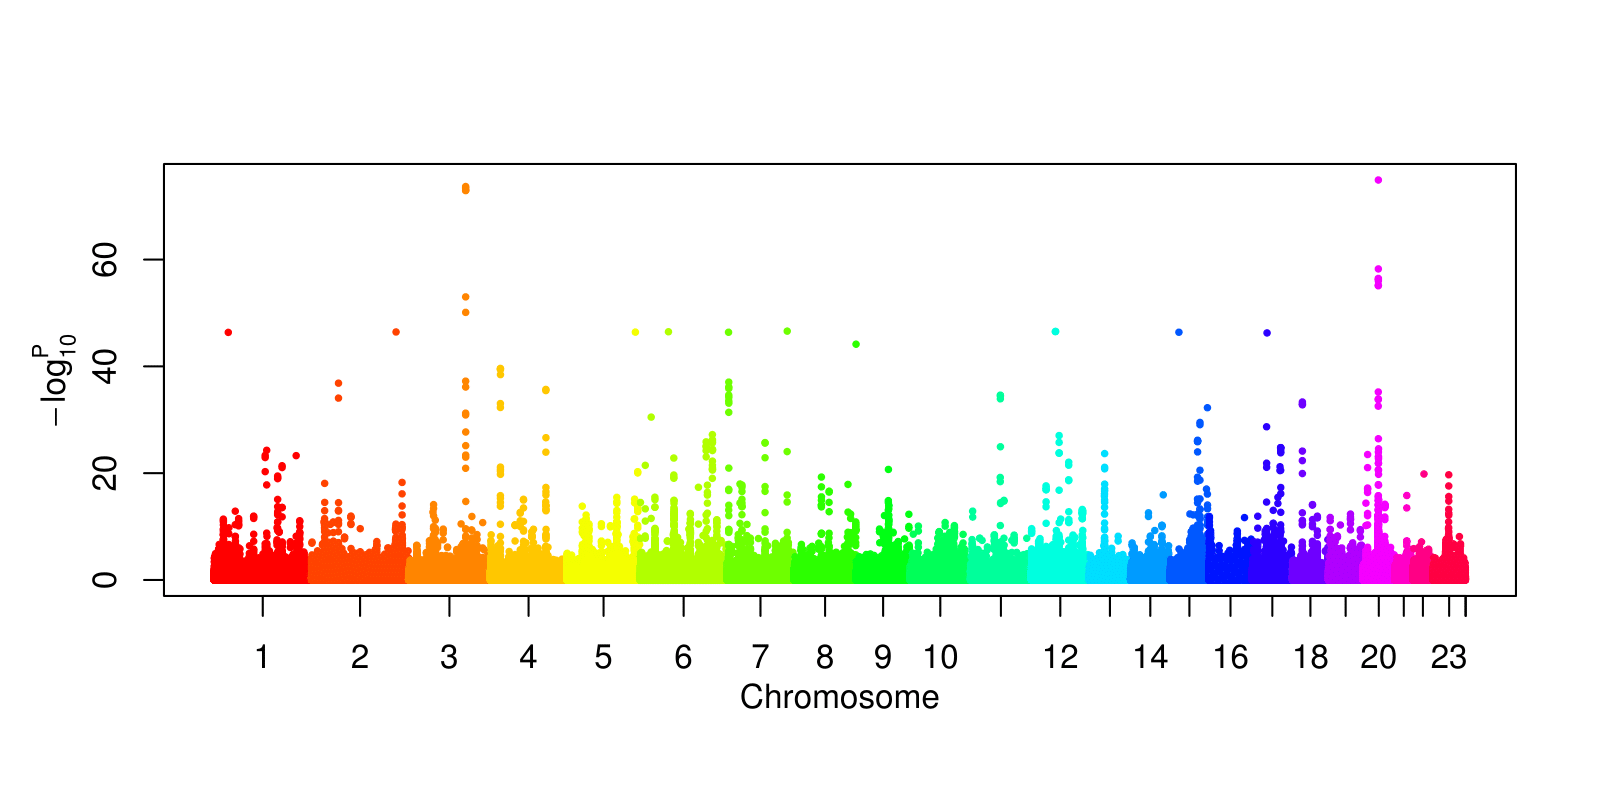
\includegraphics[width=3.5 in, trim=0 0 0in 0]{img/gwas_height}
  \caption{Negative log p-value for 600K markers.}
  \label{gwas}
\end{figure}

For each LD block, variable selection is done via four different approaches: (i) top-k selection, in which we ordered adjusted p-values descendingly in a global sense and select top k markers across whole genome; (ii) block-top-k selection, in which we selected top-k markers based on adjusted p-value within each block; (iii) stepwise selection based on information criteria, in which we use AIC and BIC to select markers within each block; (iv) selection based on LASSO in each block. Summary for selections are shown in Figure \ref{fig:AIC} and Figure {\ref{fig:BIC}}. For AIC, we end up with 123,393 selected SNPs in 80,813 blocks, while for BIC we got 6022 selected SNPs in 5554 blocks. BIC penalizes feature size more strongly than AIC and therefore tends to favor less selected markers. 

% \begin{figure}[!h]
%   \centering
%   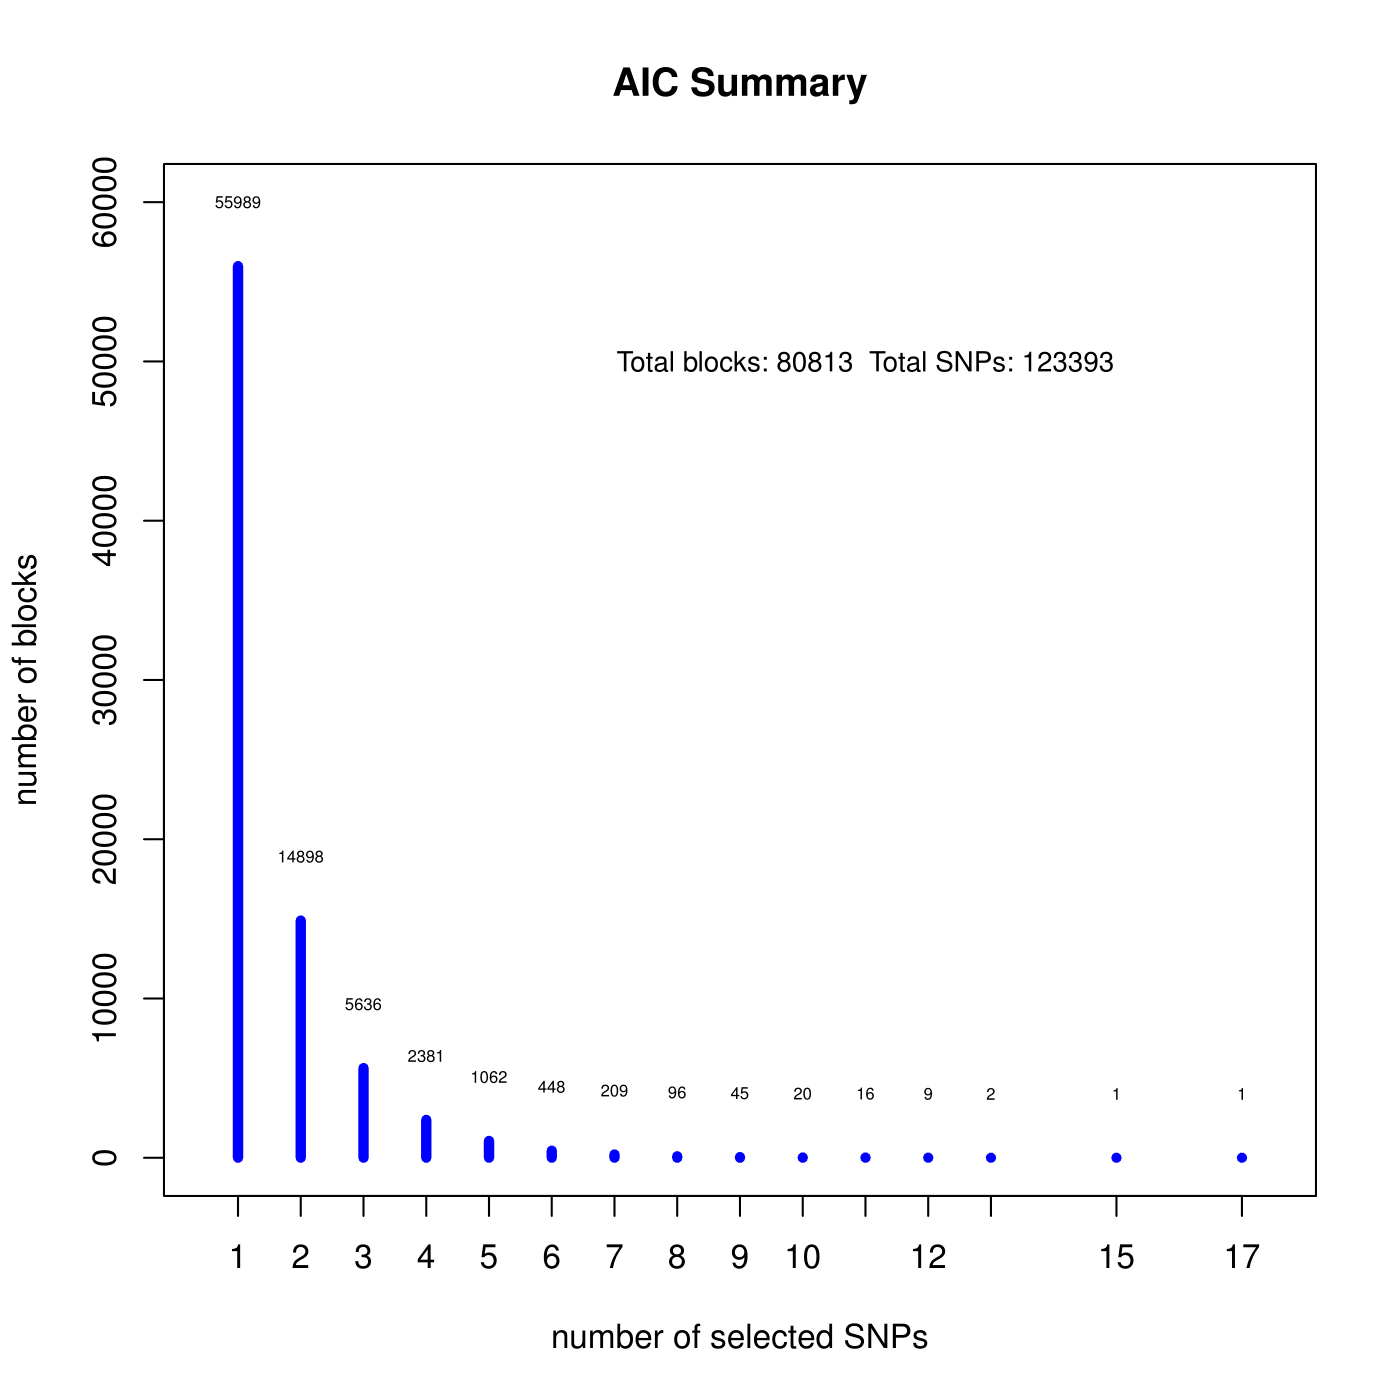
\includegraphics[width=3.5 in, trim=0 0 0in 0]{img/AIC_summary}
%   \caption{Variable selection by AIC}
%   \label{fig:AIC}
% \end{figure}
% \begin{figure}[!h]
%   \centering
%   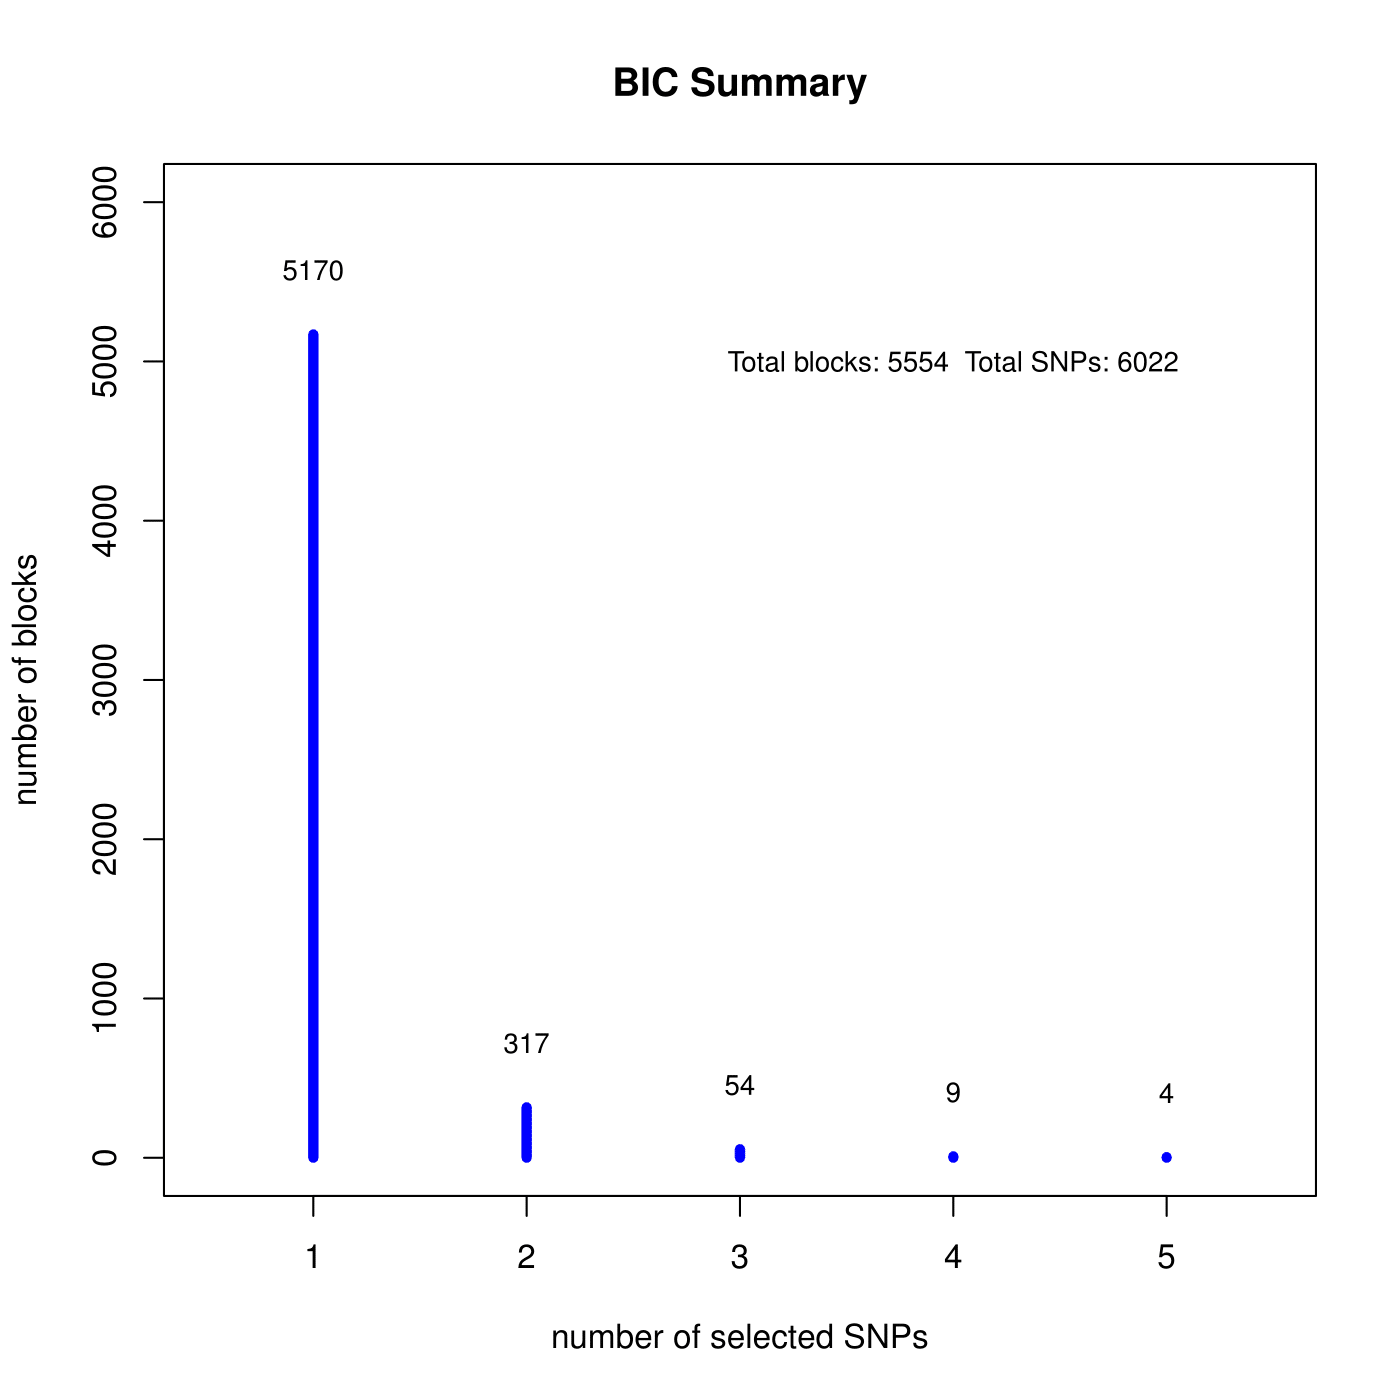
\includegraphics[width=3.5 in, trim=0 0 0in 0]{img/BIC_summary}
%   \caption{Variable selection by BIC}
%   \label{fig:BIC}
% \end{figure}


\subsection{Unsupervised Feature Extraction}
We choose stacked autoencoder(SA) \cite{DL:SDA1} to preserve non-linearity when extracting on high order feature from each superblock containing roughly 1000 raw feature. To facilitate the training, and also relax the additive genetic effect assumption, features taking count value in $\{0, 1, 2\}$ are flattened by lining up the two homogeneous chromosomes, which ends up with a double sized binary vector. At this stage we seek to overfit the encoder in order to preserve maximum information.

Before extraction though, we first benchmark the performance of sigmoid and relu autoencoders on a 2 stacking depth using randomly chosen genome segments of $512$ features ($1024$ after flattening), which is intended to find out the best configuration genomic related tasks. The overall performance is gauged by training error given the same budegt of training epochs without early stop.

The current setting halves the dimension with increasing depth, until the output become one dimensional, which gives up $1024, 512, \dots, 2, 1$ nodes in a 10 layered encoder. Both sigmoid and relu activation are tested (except the last reconstruction layer alwyas use sigmoid to restore binary feature). The mean performance of 1000 trails is shown in Figure (\ref{fig:ae0}).
\begin{figure}[h]
  \centering
  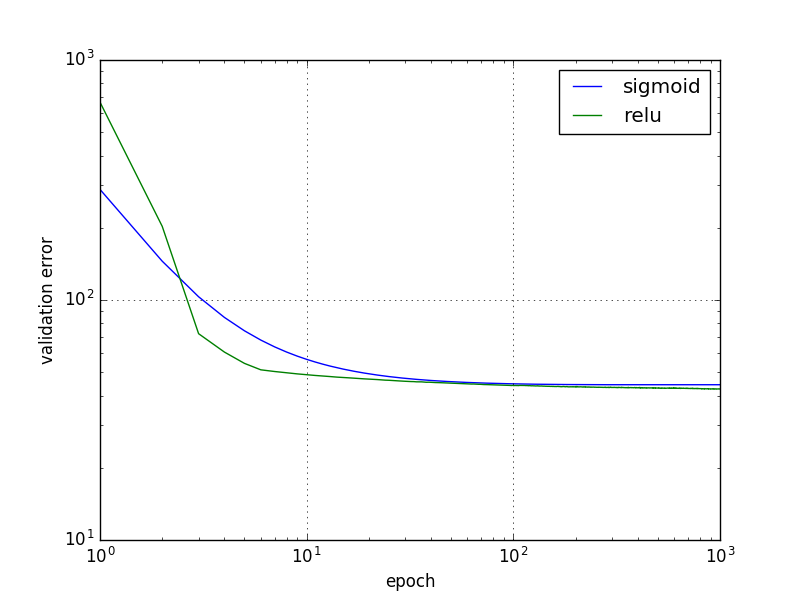
\includegraphics[width=0.35\textwidth]{img/00}
  \caption{Autoencoder Test, depth=10}
  \label{fig:ae0}
\end{figure}
We see Relu activation maintained a small edge over sigmoid networks even after long peroid of training, it also converge faster as suggested \cite{DL:Relu1}. However, the sigmoid networks did not go through the suggested layer-wise pre-train \cite{DL:Intro1} in order to make the benchmark comparable. The sigmoid activation may perform as good as Relu for a shallow SA of $10 \time 2$ layers if pre-training was done. On the other hand, Relu suffers from numerical instability due to the drastic change intermediate layers that leads to overflow, because a stack of 10 autoencoders is not deep enough to diminish the gradient that drives network change. To reduce the chance of overflow below \%0.5, we have set initial learning rate to a value as low as 1e-6, which defeat the advantages of fast convergence brought by Relu. Deeper SA network may justfy the use of Relu, but they failed to further lower the training error while demanding a significantly increase in running time. 

We decide to use classical sigmoid activation for the SAs, also implement pre-training to drive down reconstruction loss, and adapt bold driver heuristics to accelerate the training. A total of 6K superblocks were ``encoded'' to produce a 6K dimensional vector of second tier input feaures. To train such a large number of SAs, a fiew powerful GPU node is not feasible, we rely on slower but much more numerous CPU nodes on MSU HPCC instead.


% Bibliography
\bibliographystyle{ACM-Reference-Format}
\bibliography{ref}

\end{document}
